%%%%%%%%%%%%%%%%%%%%%%%%%%%%%%%%%%%%%%%%%
% Journal Article
% LaTeX Template
% Version 1.4 (15/5/16)
%
% This template has been downloaded from:
% http://www.LaTeXTemplates.com
%
% Original author:
% Frits Wenneker (http://www.howtotex.com) with extensive modifications by
% Vel (vel@LaTeXTemplates.com)
%
% License:
% CC BY-NC-SA 3.0 (http://creativecommons.org/licenses/by-nc-sa/3.0/)
%%%%%%%%%%%%%%%%%%%%%%%%%%%%%%%%%%%%%%%%%

%----------------------------------------------------------------------------------------
%	PACKAGES AND OTHER DOCUMENT CONFIGURATIONS
%----------------------------------------------------------------------------------------

\documentclass[twoside,twocolumn]{article}

\usepackage[utf8]{inputenc}

\usepackage{blindtext} % Package to generate dummy text throughout this template

\usepackage[sc]{mathpazo} % Use the Palatino font
\usepackage[T1]{fontenc} % Use 8-bit encoding that has 256 glyphs
\linespread{1.05} % Line spacing - Palatino needs more space between lines
\usepackage{microtype} % Slightly tweak font spacing for aesthetics

\usepackage[german]{babel} % Language hyphenation and typographical rules

\usepackage[hmarginratio=1:1,top=32mm,columnsep=20pt]{geometry} % Document margins
\usepackage[hang, small,labelfont=bf,up,textfont=it,up]{caption} % Custom captions under/above floats in tables or figures
\usepackage{booktabs} % Horizontal rules in tables

\usepackage{lettrine} % The lettrine is the first enlarged letter at the beginning of the text

\usepackage{enumitem} % Customized lists
\setlist[itemize]{noitemsep} % Make itemize lists more compact

\usepackage{abstract} % Allows abstract customization
\renewcommand{\abstractnamefont}{\normalfont\bfseries} % Set the "Abstract" text to bold
\renewcommand{\abstracttextfont}{\normalfont\small\itshape} % Set the abstract itself to small italic text

\usepackage{titlesec} % Allows customization of titles
\renewcommand\thesection{\Roman{section}} % Roman numerals for the sections
\renewcommand\thesubsection{\roman{subsection}} % roman numerals for subsections
\titleformat{\section}[block]{\large\scshape\centering}{\thesection.}{1em}{} % Change the look of the section titles
\titleformat{\subsection}[block]{\large}{\thesubsection.}{1em}{} % Change the look of the section titles

\usepackage{fancyhdr} % Headers and footers
\pagestyle{fancy} % All pages have headers and footers
\fancyhead{} % Blank out the default header
\fancyfoot{} % Blank out the default footer
\fancyhead[C]{Evolutionäre Optimierungsalgorithmen $\bullet$ MK - Einführung in das wissenschaftliche Arbeiten} % Custom header text
\fancyfoot[RO,LE]{\thepage} % Custom footer text

\usepackage{titling} % Customizing the title section

\usepackage{hyperref} % For hyperlinks in the PDF

\newcommand{\e}[1]{\times 10^{#1}}

\usepackage{graphicx}

\usepackage{amsmath}

\usepackage{csquotes}

%----------------------------------------------------------------------------------------
%	TITLE SECTION
%----------------------------------------------------------------------------------------

\setlength{\droptitle}{-4\baselineskip} % Move the title up

\pretitle{\begin{center}\Huge\bfseries} % Article title formatting
\posttitle{\end{center}} % Article title closing formatting
\title{Evolutionäre Optimierungsalgorithmen} % Article title
\author {
	\textsc{Federico Ramírez Villagrana} \\[1ex]
	\normalsize Universität Hamburg \\
	\normalsize Methodenkompetenz - Einführung in das wissenschaftliche Arbeiten \\
	\normalsize Dozent: Dr. Andreas Günther
}
\date{} % Leave empty to omit a date
\renewcommand{\maketitlehookd}{%
\begin{abstract}
\noindent In dieser Arbeit wird darüber diskutiert, sowohl was Optimierung ist und warum es schwierig ist, als auch was evolutionäre Algorithmen (EA) sind und wie, warum,  und wann sie hilfreich im Optimierungsbereich sind. Es wird auch detailliert, wie EA funktionieren und warum sie als teil der künstlichen Intelligenz betrachtet werden. Es werden auch einige bekannte EA erwähnt und kurz erläutert erklärt. Am Ende wird darüber diskutiert, welche Vor- und Nachteile EA haben können.
\end{abstract}
}

%----------------------------------------------------------------------------------------

\begin{document}

% Print the title
\maketitle

%----------------------------------------------------------------------------------------
%	ARTICLE CONTENTS
%----------------------------------------------------------------------------------------

\section{Einleitung}
Das Problem des Handlungsreisenden (engl. traveling salesman problem oder TSP) ist ein sehr bekanntes und studiertes Thema in den Informatik- und Optimierungsbereich. Es sieht folgendermaßen aus:\par
Eine Reihenfolge für den Besuch mehrerer Orte muss so gewählt sein, dass keine Station, außer der ersten, mehr als einmal besucht wird, die gesamte Reisestrecke des Handlungsreisenden möglichst kurz ist, und die erste Station gleich wie die letzte Station ist \cite{wiki_tsp}.\par
Sei $n$ die Anzahl der Stationen, dann gibt es $(n-1)!$ mögliche Lösungen für das TSP. Daher wenn $n=4$, dann gibt es $6$ mögliche Lösungen. Es ist nicht schwierig, einen brute-force \footnote{Auch Exhaustionsmethode, ist eine Lösungsmethode für Probleme, die auf dem Ausprobieren aller möglichen (oder zumindest vieler möglicher) Fälle beruht \cite{wiki_brute_force}.} Ansatz zu verfolgen, für ein Problem, das nur 6 Lösungen hat. Aber wenn $n=50$, dann gibt es circa $6,1\e{62}$ Lösungen.\par
Folgendes ist hilfreich, um diese Anzahl in einer Perspektive zu setzen: Das Universum ist circa 15 Milliarde Jahre alt, das ist $4,7\e{17}$ Sekunden. Wenn es eine Billion Rechner gäbe, die jede seit Anfang des Universums eine Billion Lösungen pro Sekunde berechnen würde, so wären bisher nur $4,7\e{41}$ Lösungen berechnet worden.\par
Das TSP ist nur ein Beispiel des vielfältigen Probleme, die zu den kombinatorischen Problemen gehören, das heißt: Probleme, für die kein brute-force Ansatz möglich ist. In diesem Fall sind evolutionäre Algorithmen (EA) ein sinnvolles Werkzeug, um optimale Lösungen zu finden.\par
Natürlich kann man nicht sicher sein, dass man die beste Lösung gefunden hat, außer würde man jede mögliche Lösung berechnen. Aber wie mit dem TSP-Beispiel gezeigt worden, kann man nicht immer alle mögliche Lösungen (in angemessener Zeit) berechnen.

%------------------------------------------------

\section{Stand der Forschung}
In den 70ern Jahren wurde erstmals über EA diskutiert. Die erste Form von EA waren die genetischen Algorithmen, die in \cite{holland_ga} eingeführt wurden. Seitdem wurden jedes Jahr mehrere EA vorgestellt. Es ist auch üblich, dass nicht nur Varianten von schon bekannten EA, sondern auch neue Anwendungen eingeführt werden. In \cite{algorithmen_list} allein werden circa 48 EA gelistet.\par
Heutzutage finden sich immer mehr Anwendungen der EA in nahezu allen Bereichen. Von der Medizin \cite{ea_und_medizin} und Biologie \cite{ea_und_biologie} über das Motor- \cite{ea_und_motoren} und Flugzeugdesign \cite{ea_und_flugzeuge_a} \cite{ea_und_flugzeuge_b} bis hin zur Kunst \cite{ea_und_kunst_a} \cite{ea_und_kunst_b} und Wirtschaft \cite{ea_und_wirtschaft}.

%------------------------------------------------

\section{Optimierung}
Im Bereich der Mathematik bedeutet Optimierung, die Findung von Parametern eines Systems, die ein bestmögliches Ergebnis erzielen sollen. \cite{wiki_optimierung} Wir können diese Findung von Parametern auch folgendermaßen definieren: Die Auswahl der bestmöglichen Lösungen eines Problems aus einer Menge möglicher Lösungen.\par
Bei Optimierungsproblemen wird eine Zielfunktion (engl. objective function) definiert, die entweder maximiert oder minimiert werden soll. Die Zielfunktion wird \enquote{Kosten-Funktion} oder \enquote{Fitness-Funktion} in Minimierung- und Maximierungsprobleme genannt.\par
Sei $f(x)$ eine Zielfunktion, und $x$ ein Vektor, der \enquote{Entscheidungsvariable} genannt wird. Die Anzahl an Elementen in $x$ wird die \enquote{Dimension} des Problems genannt.
Die Domäne der Zielfunktion repräsentiert die möglichen Lösungen des Problems. \par
Das Ziel der Optimierung ist es, die bestmögliche Lösung des Problems zu finden, das heißt, einen Wert für die Entscheidungsvariable zu finden, sodass die Zielfunktion einen Maximal- beziehungsweise Minimalwert ergibt.\par
Es gibt verschiedene Klassifizierungen oder Arten von Optimierung:

\begin{itemize}
\item{\textbf{Eingeschränkte Optimierung} - Die Entscheidungsvariable kann nicht irgendwelche Werte aus der Domäne der Zielfunktion nehmen. Es gibt Einschränkungen dafür.}
\item{\textbf{Multi-objective Optimierung} - Das Problem besteht aus vielfältigen Zielfunktionen.}
\item{\textbf{Multi-modale Optimierung} - Die Zielfunktion hat mehrere Minima bzw. Maxima. Abbildung \ref{fig:rastrigin} zeigt eine multi-modale Funktion.}
\end{itemize}

\begin{figure}
\caption{Rastrigin function. Quelle: \url{https://commons.wikimedia.org/wiki/File:Rastrigin_function.png}}
\label{fig:rastrigin}
\centering
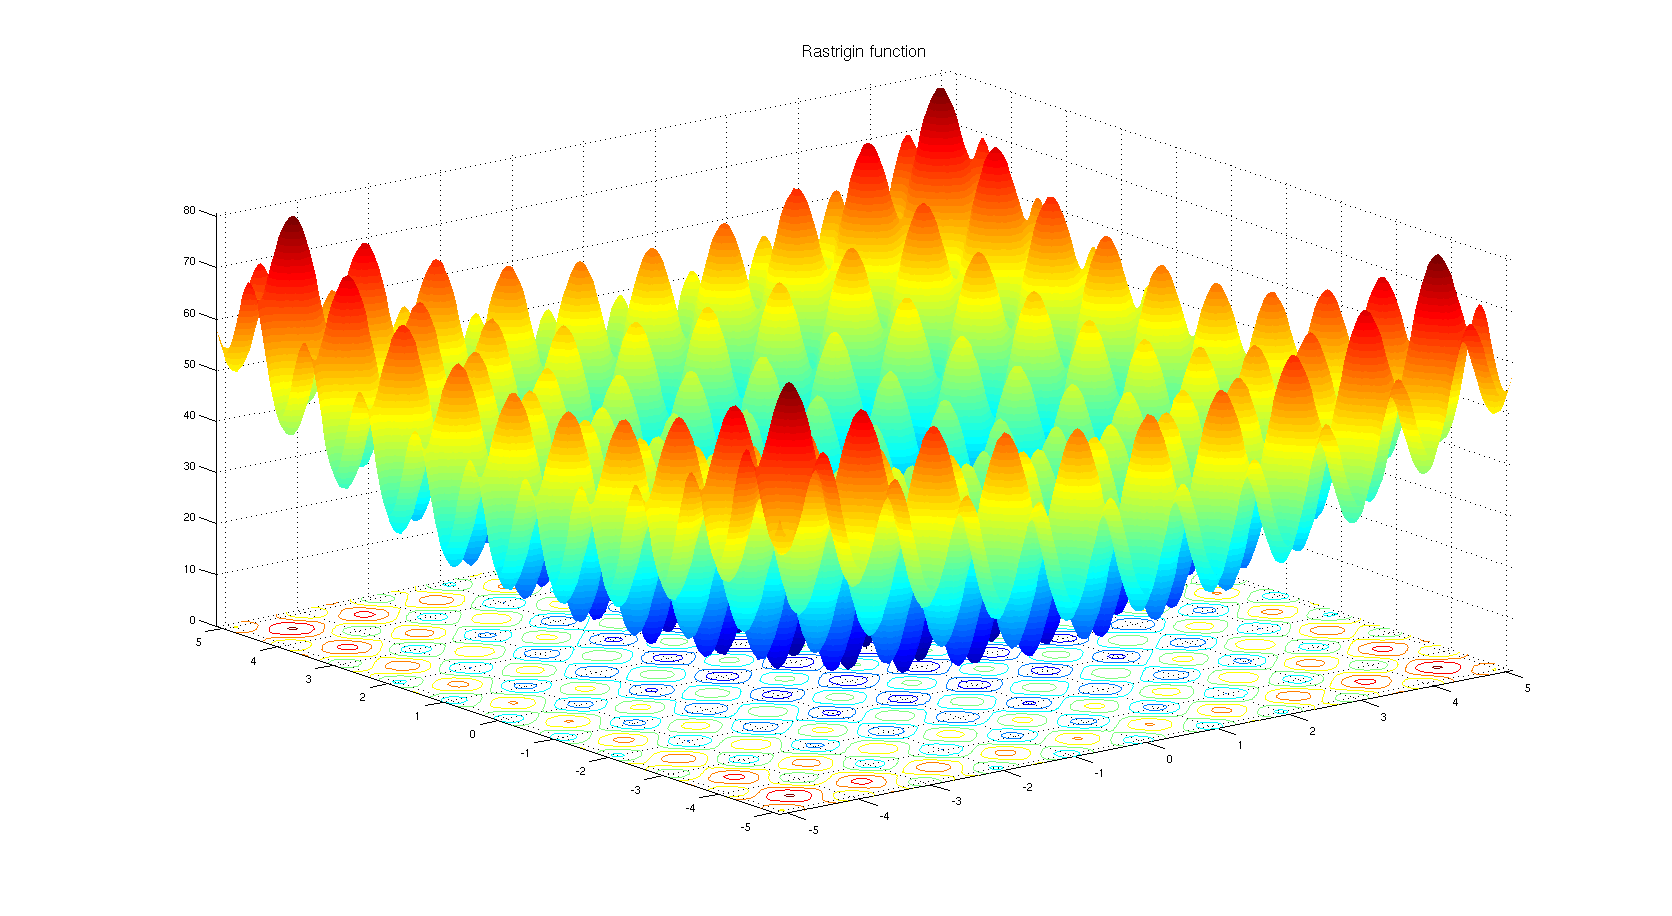
\includegraphics[width=0.5\textwidth]{images/rastrigin_function.png}
\end{figure}

Eine der wichtigsten und schwierigsten Teile der Optimierung ist es, eine geeignete Zielfunktion zu definieren, die die wichtige zu optimierenden Faktoren berücksichtigt.
Probleme im wirklichen Leben sind normalerweise eingeschränkt, multi-objectiv und multi-modal, oder haben eine große Anzahl an Dimensionen. Wegen dieser Eigenschaften der Zielfunktionen und der Optimierungsprobleme ist es schwierig eine gute Lösung mittels traditioneller Vorgänge zu finden. Im Laufe der Zeit haben EA sich als gutes Werkzeug zur Lösung dieser Art von Probleme in angemessener Zeit erwiesen.

%------------------------------------------------

\section{Was ist ein evolutionärer Algorithmus?}
Der EA-Bereich ist ziemlich neu, deswegen gibt es bisher keine allgemein akzeptierte Definition des evolutionären Algorithmus.\par
EA werden zwar als Teil der künstliche Intelligenz (KI) betrachtet, aber genau wo sie in Verbindung mit anderen KI-Methoden stehen, und was der EA-Bereich beinhaltet, ist vom Autor abhängig. Abbildung \ref{fig:metaheuristics} zeigt eine von mehreren möglichen Klassifikationen von KI-Methoden in Bezug auf Metaheuristics (welche über den Rahmen dieser Arbeit hinausgehen).

\begin{figure}
\caption{Klassifikation von Metaheuristics. Quelle: \url{https://en.wikipedia.org/wiki/File:Metaheuristics_classification.svg}}
\label{fig:metaheuristics}
\centering
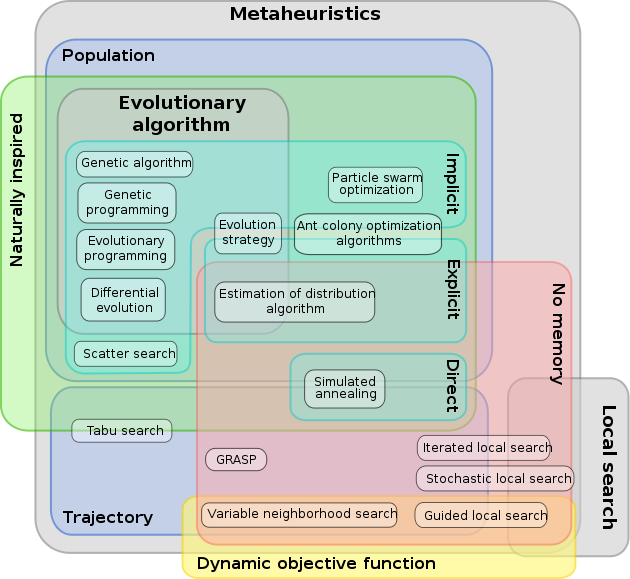
\includegraphics[width=0.5\textwidth]{images/metaheuristics_classification.png}
\end{figure}

In Abbildung \ref{fig:metaheuristics} kann auch erkannt werden, dass der Autor Particle Swarm Optimization (PSO) und Ant Colony Optimization (ACO) nicht als EA betrachtet. Trotzdem gibt es andere Autoren (wie z. B. \cite{wiley_evolutionary}), die diese Algorithmen genau für EA halten.\par

In dieser Arbeit wird folgende Definition für evolutionärer Algorithmus herangezogen: \textit{Ein Algorithmus, der die Lösung eines Problems durch viele Iterationen entwickelt}.

\subsection{Eigenschaften der evolutionären Algorithmen}
Folgende sind die Hauptelemente, die ein Algorithmus haben soll, damit es als \enquote{evolutionär} betrachten werden kann:

\begin{itemize}
\item{\textbf{Eine Zielfunktion} - Der Wert, den ein Element der Bevölkerung darstellt, wird die Eingabe für die Zielfunktion. Der Wert, den die Zielfunktion ergibt, wird als \enquote{Fitness} oder \enquote{Kosten} des Elements bezeichnet}
\item{\textbf{Eine sogenannte Bevölkerung von mögliche Lösungen} - Eine Menge von Darstellungen der Lösungen (Elemente der Domäne der Zielfunktion) des Problems, die mittels des Algorithmus und mehreren Iterationen (auch \enquote{Generationen} genannt) verarbeitet und verbessert werden.}
\item{\textbf{Vorgänge, die die Elementen der Bevölkerung betreffen und verändern.}}
\end{itemize}

Die meisten EA sind aus der Natur inspiriert, das heißt, dass WissenschaftlerInnen Ereignisse, Systeme, und Mechanismen der Natur beobachten und danach versuchen, sie mit Algorithmen zu emulieren. EA werden \enquote{evolutionär} genannt, denn sie ursprünglich auf der Evolution basieren. \cite{holland_ga}

\subsection{Eigenschaften der Intelligenz}
Wie bereits erwähnt, EA werden als Teil der KI zu betrachten, weil sie Eigenschaften intelligenter natürlicher Systeme emulieren.\par
Laut \cite[Kapitel 2.7]{wiley_evolutionary} sind die folgenden Eigenschaften notwendig, um ein System als intelligent zu betrachten:

\begin{itemize}
\item{\textbf{Adaptation} - Ein intelligentes System muss in hohem Maße an unvorhersehbare Änderungen anpassbar sein. Lernen ist daher unerlässlich.}
\item{\textbf{Zufälligkeit} - Obwohl Zufälligkeit meistens als eine schlechte Eigenschaft betrachtet wird, ist es in gewissem Maße notwendig, damit neue Lösungen eines Problems gefunden werden können.}
\item{\textbf{Kommunikation} -  Zwar wird eine einzige Ameise nicht als intelligent gesehen, aber eine Ameisenkolonie wird (dank Kommunikation durch Pheromone) als eine super-intelligente Einheit betrachtet.}
\item{\textbf{Rückmeldung} - Ein System kann sich nicht anpassen und verbessern, wenn es seine Umgebung nicht erkennen und darauf reagieren kann. Auch um zu erlernen, muss ein System seine Fehler (mittels Rückmeldung) erkennen.}
\item{\textbf{Erkundung} - Das heißt, neue Lösungen finden, neue Wege erkunden, neue Ideen erzeugen. Normalerweise ist Erkundung eng mit Zufälligkeit verbunden.}
\item{\textbf{Ausbeutung} - Das Gegenteil von Erkundung. Das heißt, schon bekannte Lösungen und Wege (oder Kenntnisse) ausnutzen.}
\end{itemize}

%------------------------------------------------

\section{EA Beispiele}
Heutzutage gibt es viele EA und jedes Jahr werden neue entwickelt. In dieser Sektion werden nur ein paar der bekanntesten und wichtigsten erwähnt und kurz erklärt.

\subsection{Genetische Algorithmen}
Genetische Algorithmen (engl. genetic algorithms oder GA) sind ursprünglich in \cite{holland_ga} präsentiert und danach in \cite{goldberg_ga} weiterentwickelt. Der Name \enquote{Genetic Algorithms} bezieht sich mehr auf eine Familie von Algorithmen als auf einen einzigen Algorithmus.\par
GA sind die ersten vorgestellten, bekanntesten und am meisten verwendeten EA. Ursprünglich waren sie dafür entwickelt um adaptierbare Systeme zu studieren. Sie sind Simulationen der natürlichen Selektion. Überdies versuchen sie die Evolution zu simulieren.\par
Folgende sind die Hauptteile der GA:

\begin{enumerate}
\item{\textbf{Codierung der Lösungen} - Als erstes muss man eine geeignete Codierung für die möglichen Lösungen finden. Das heißt, eine einfach zu verarbeitende Darstellung für die Lösungen zu definieren. Die am häufigsten verwendeten Codierungen sind eine Bitfolge und ein Vektor reeller Zahlen. In diesen Codierungen wird jedes Bit beziehungsweise reelle Zahl \enquote{Gen} genannt.}
\item{\textbf{Ursprüngliche Bevölkerung} - Eine ursprüngliche Bevölkerung muss initialisiert werden. Diese Initialisierung kann entweder zufällig oder auf Vorkenntnis basiert werden. Wie viele Elemente die Bevölkerung hat, ist ein wichtiger Parameter. Je mehr Elemente es gibt desto, höher ist die Wahrscheinlichkeit um geeignete Lösungen zu finden, und desto geringer ist der Zeitaufwand.}
\item{\textbf{Auswahl von Einzelnen} - Zwei Elemente der Bevölkerung werden ausgewählt, um ein neues Element herzustellen. Das verfolgte Verfahren, um die Elemente auszuwählen, kann entweder zufällig sein, oder auf der Fitness der Elemente basieren. Die ausgewählten Elemente werden \enquote{Eltern} genannt.}
\item{\textbf{Crossover} - Dies ist der wichtigste Teil der GA. Es definiert wie ein neues Element aus den Eltern erstellt wird. Das heißt, welche Gene die neuen Elemente von jedem Elternteil erben werden.}
\item{\textbf{Mutation} - Einige per Zufall ausgewählte neu erstellte Elemente werden mutiert. Das heißt, dass einige Bits gekippt werden. Welche Elemente mutiert werden und wie viele und welche Bits gekippt werden, kann mittels verschiedener Verfahren entschieden werden.}
\end{enumerate}

\begin{figure}
\caption{Wesentlich genetic Algorithmen pseudo-Code. Quelle: \cite[p.~50]{wiley_evolutionary}}
\label{fig:ga_pseudo}
\centering
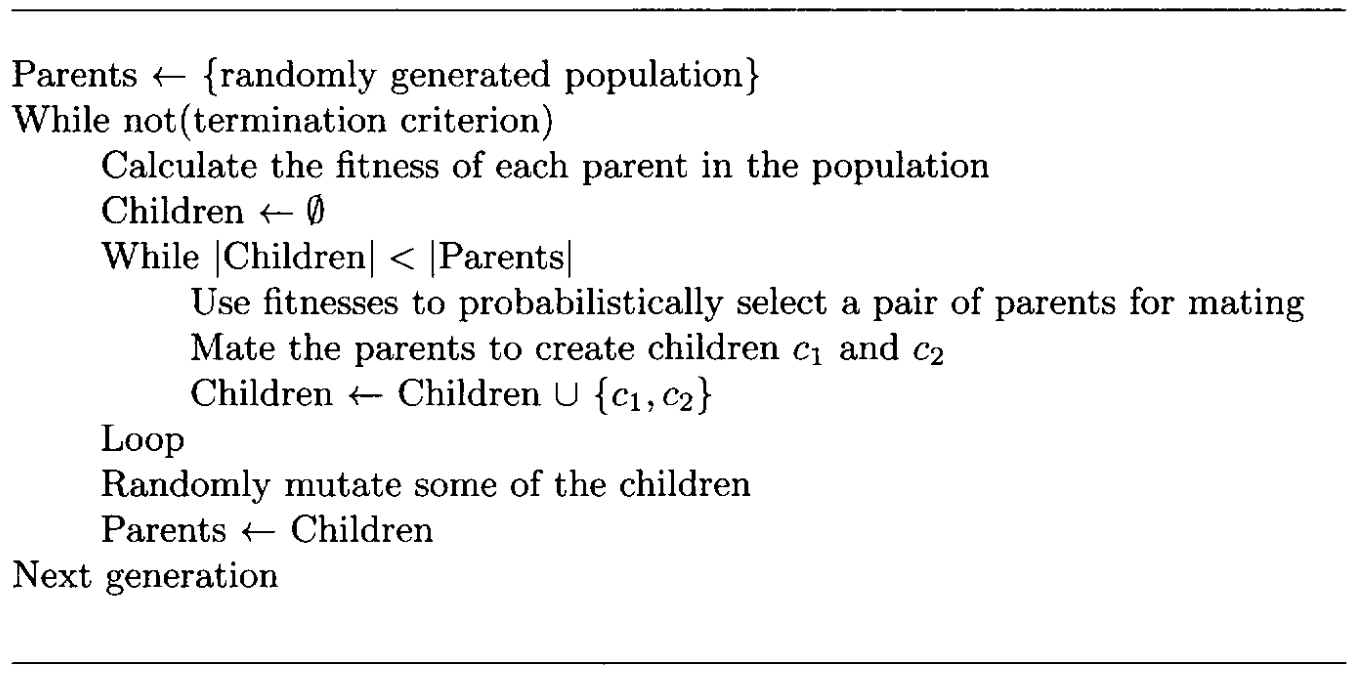
\includegraphics[width=0.5\textwidth]{images/ga_pseudo.png}
\end{figure}

EA sind insgesamt Problem-unabhängig, das bedeutet, dass wenn es eine geeignete Darstellung der Lösungen und eine geeignete Zielfunktion gibt, kann theoretisch jedes Problem mittels EA optimiert werden. Aus diesem Grund gibt es bei jeden EA ein Element der \textbf{Adaptation}.\par
In allen Teile der GA außer die Erste kann \textbf{Zufälligkeit} verwendet werden, je nachdem welche Verfahren jeweils ausgewählt werden. In dem Mutationsteil, eine hohe Wahrscheinlichkeit, um Elemente zu mutieren, heißt viel \textbf{Erkundung} und weniger \textbf{Ausbeutung}, während eine geringe Wahrscheinlichkeit bedeutet viel \textbf{Ausbeutung} und weniger \textbf{Erkundung}.

\subsection{Partikelschwarmoptimierung}
Partikelschwarmoptimierung (engl. particle swarm optimization oder PSO) wird ursprünglich in \cite{kennedy_pso} und in \cite{shi_pso} präsentiert.\par
PSO basiert auf menschlichen sozialen Verhalten. \cite{eberhart_pso} Genauer gesagt, PSO basiert auf der Beobachtung von Gruppen von Individuen, die zusammenarbeiten, um nicht nur ihr kollektives Verhalten in einer bestimmten Aufgabe zu verbessern, sondern auch ihr individuelles Verhalten zu verfeinern.\par
Die Grundidee hinter PSO ist die folgende:

\begin{itemize}
\item{Es gibt eine Menge von Partikeln, die sich mit einer beliebigen Geschwindigkeit durch den Suchraum bewegen.}
\item{Der Suchraum wird in \enquote{Nachbarschaften} mit einer beliebigen Größe unterteilt.}
\item{Jede Partikel speichert sowohl die beste Position, die sie im Suchraum besucht hat, als auch die beste Position, die ihre Nachbarn erreichen haben.}
\item{Sowohl die beste Position des Partikels, als auch die der Nachbarn beeinflussen die Geschwindigkeit des Partikels.}
\end{itemize}

\begin{figure}
\caption{Wesentlich PSO Algorithmus pseudo-Code. Quelle: \cite[p.~268]{wiley_evolutionary}}
\label{fig:pso_pseudo}
\centering
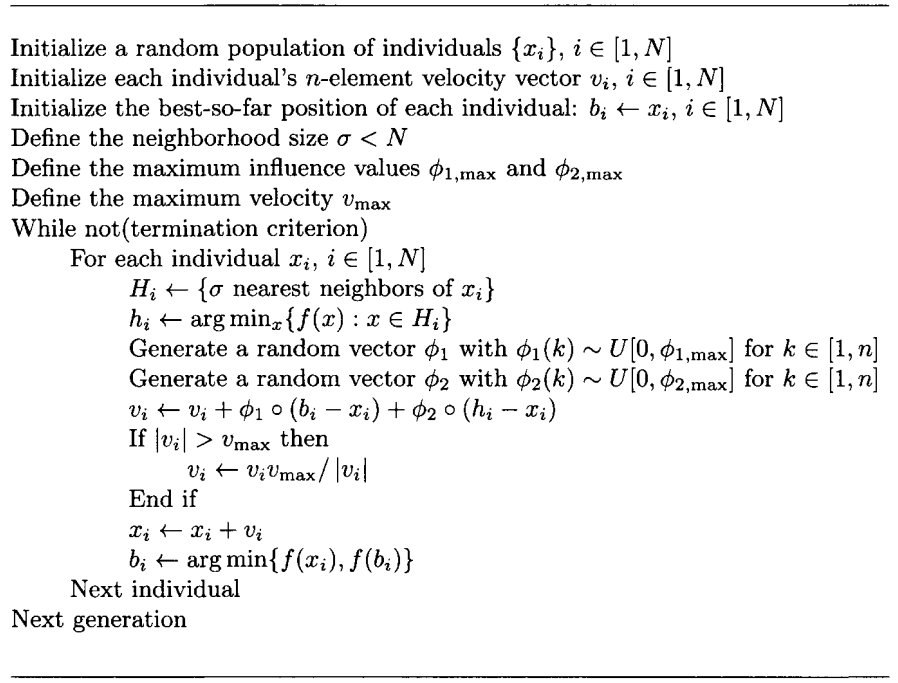
\includegraphics[width=0.5\textwidth]{images/pso_pseudo.png}
\end{figure}

In PSO können die Geschwindigkeiten der ersten Bevölkerung zufällig initialisiert werden. Daher gibt es ein Element der \textbf{Zufälligkeit}. Da die Partikeln, die besten bisher erreichten Positionen ihrer Nachbarn kennen müssen, gibt es auch \textbf{Kommunikation}. \textbf{Rückmeldung} wird verwendet, indem die besten bisher erreichten Positionen die Geschwindigkeit der Partikel beeinflussen. In welchem Ausmaß die Partikel beeinflusst wird, kann entweder \textbf{Erkundung} oder \textbf{Ausbeutung} fördern.

\subsection{Differenziale Evolution}
Differenziale Evolution (engl. differential evolution oder DE) wurde erstmals in \cite{storn_de_a} und \cite{storn_de_b} erwähnt. Aber die erste vielfach gelesene DE-Veröffentlichung war \cite{price_storn_de}.\par
Im Gegensatz zu fast allen anderen EA, ist DE nicht nach der Natur inspiriert. Eine der wichtigsten Merkmale der DE ist, dass es einfach ist. Dieses Merkmal ist wichtig, da es Benutzer aus anderen Bereiche (d. h. nicht InformatikernInen oder MathematikerInen) erlaubt, es umzusetzen.\par
Die wesentliche Schritte eines DE Algorithmus sind die folgende:

\begin{enumerate}
\item Die Bevölkerung eines DE Algorithmus besteht aus Vektoren mit $n$ Elemente. Wobei $n$ die Dimension des Problems ist. Weiterhin stellt jeder Vektor selbst eine mögliche Lösung des Problems dar.
\item Zwei Vektoren $x_{r2}, x_{r3} \mid r2 \neq r3$ werden ausgewählt.
\item Die Differenz zwischen $x_{r2}$ und $x_{r3}$ wird berechnet.
\item Die skalierte Differenz wird zu einem dritten Vektor $x_{r1} \mid r1 \notin \{ r2, r3 \}$ addiert. Daraus wird sich eine neue mögliche Lösung $v_i$ ergeben.
\item $v_i$ wird mit einem Vektor $x_i \mid i \notin \{ r1, r2, r3 \}$ kombiniert.
\item Die Fitness von $x_i$ und $u_i$ werden vergleichen und nur den Vektor mit die besten Fitness wird behalten.
\end{enumerate}

Abbildung \ref{fig:de_beispiel} zeigt 2. bis 4. Schritte für ein Problem mit 2 Dimensionen. Abbildung \ref{fig:de_pseudo} zeigt einen kompletten DE Algorithmus pseudo-Code für $n$ Dimensionen.\par

\begin{figure}
\caption{Grundlegende Idee der DE. Quelle: \cite[p.~294]{wiley_evolutionary}}
\label{fig:de_beispiel}
\centering
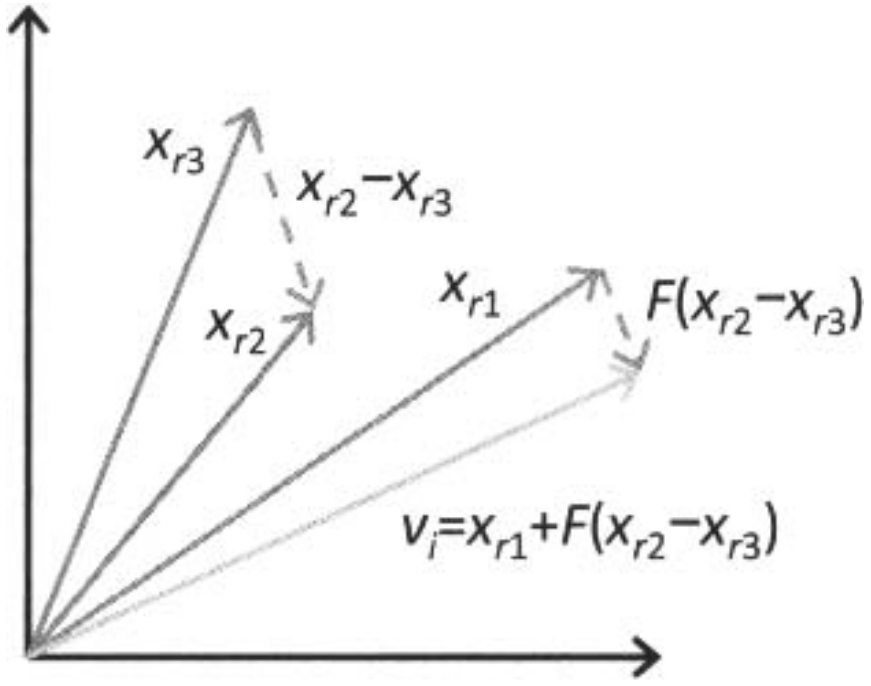
\includegraphics[width=0.5\textwidth]{images/de_beispiel.png}
\end{figure}

\begin{figure}
\caption{Wesentlich DE Algorithmus pseudo-Code. Quelle: \cite[p.~295]{wiley_evolutionary}}
\label{fig:de_pseudo}
\centering
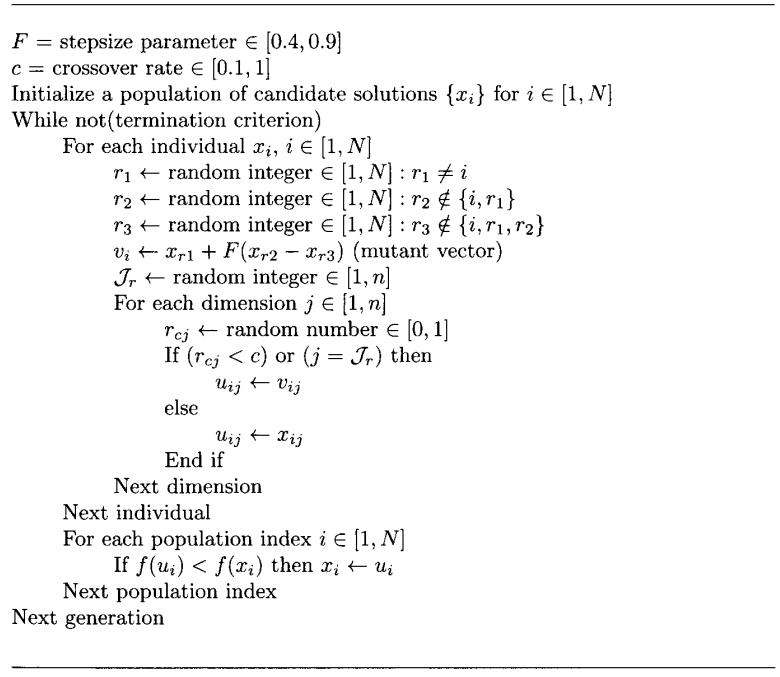
\includegraphics[width=0.5\textwidth]{images/de_pseudo.png}
\end{figure}

Der Algorithmus, den die Abbildung \ref{fig:de_pseudo} beschreibt, wird \enquote{DE/rand/1/bin} genannt und stellt die einfachste Variante der DE Algorithmen dar. Andere Varianten sind zum Beispiel \enquote{DE/best/1/L}, \enquote{DE/best/2/bin}, \enquote{DE/rand/1/exp}.\par
Jeder Teil dieser Namen bezieht sich auf die Verfahren, die für bestimmte Schritte der DE Algorithmen verwendet werden.\par
Zum Beispiel der \enquote{rand/best}-Teil\footnote{\enquote{best} und \enquote{rand} sind nicht die einzige Varianten.} beschreibt wie Vektoren $x_{r1}$ und $x_{r2}$ im 2. Schritt ausgewählt werden. \enquote{rand} bedeutet, dass die Vektoren per Zufall ausgewählt werden, während \enquote{best} heißt, dass die beste Vektoren eine höhere Wahrscheinlichkeit haben, um ausgewählt zu werden.\par
In \cite{love_u_mex} werden die Leistungen mehrerer Varianten von DE Algorithmen verglichen.\par
Wenn Vektoren $x_{r1}$ und $x_{r2}$ zufällig ausgewählt werden, gibt es ein Element der \textbf{Zufälligkeit}. Wenn nur die besten Vektoren ausgewählt werden, wird \textbf{Ausbeutung} gefördert. Die Tatsache, dass nur der beste Vektor im 6. Schritt behalten wird, zeigt die Verwendung von \textbf{Rückmeldung}. Die Kombination, die im 5. Schritt stattfindet, könnte auch entweder \textbf{Erkundung} oder \textbf{Ausbeutung} fördern.

%------------------------------------------------

\section{Diskussion}
\subsection{Vor- und Nachteile}
Der größte Vorteil der evolutionären Algorithmen ist, dass es praktisch keine Grenze für ihren Verwendungsbereich gibt. Wie bereits besprochen, wenn es eine geeignete Darstellung der Lösungen eines Problems gibt, und eine geeignete Zielfunktion sich definieren lässt, kann jedes Problem mit EA optimiert werden.\par
Im Vergleich mit anderen Lösungsmethoden sind EA vorteilhafter, denn sie annehmbare Lösungen in weniger Zeit und mit geringen Gesamtaufwand finden können.\par
Ein Nachteil der EA ist, dass die Definition einer geeigneten Zielfunktion ein Problem gleicher Größe wie das Ursprüngliche darstellen könnte. Dies ist vermeidbar, indem das Problem geteilt wird. In der Praxis werden oft EA verwendet, um mehrere separate Teile großer komplexer Systeme zu optimieren.\par
Ein weiteres Nachteil der EA ist, dass die Einstellung der Parametern der Algorithmen auch ein großes Problem darstellen könnte. Die Leistung der Algorithmen ist in großen Anteil davon abhängig, wie die ursprüngliche Bevölkerung initialisiert wird, und welche Werte für die Parametern der Algorithmen ausgewählt werden. Dies ist zu einem so großen Problem geworden, dass dazu Forschung betrieben wird. Um einige Beispiele zu nennen, \cite{pso_tuning_a} und \cite{pso_tuning_c} stellen Verfahren zur Parametereinstellung für PSO vor.\par
EA sollten immer berücksichtigt werden, wenn ein schwieriges Optimierungsproblem gelöst werden soll. Das bedeutet aber nicht, dass EA immer die beste Wahl sind; Wenn eine Gebäude oder ein komplexes Transportsystem projektiert werden soll, dann sind EA ein geeignetes Werkzeug; wenn eine komplexe elektrische Schaltung oder ein Computerprogramm entworfen werden soll, dann können EA die Aufgabe erfüllen; Aber wenn das Problem jedoch mit klassischen Methoden, analytisch oder numerisch, eine annehmbare Lösung bietet, ist es besser, diese Methoden zu verwenden.

\subsection{Vergleich mit anderen Methoden}
Optimierungsprobleme wurden seit lange umfassend untersucht, auf diesem Grund gibt es viele verschiedene Ansätze und Techniken, um sie versuchen zu lösen. Hier wird das Problem des Handlungsreisenden wieder genommen, um verschiedene Optimierungsprobleme-Lösungsmethoden zu vergleichen.\par
Es gibt zwei Kategorien, in denen Optimierungsprobleme-Lösungsverfahren eingeordnet werden können.
\begin{itemize}
\item{\textbf{Exakte Algorithmen} - Algorithmen, die genau die beste Lösung eines Problems finden. Diese Algorithmen haben ein große rechnerisch Aufwand, denn sie (implizit) alle mögliche Lösungen berücksichtigten müssen, um die Beste zu identifizieren.}
\item{\textbf{Heuristische Algorithmen} - Diese Algorithmen, finden annehmbare Lösungen dank der Nutzung von Heuristiken. Normalerweise sind solche Algorithmen weder Zeit- noch rechnerisch-aufwendig.}
\end{itemize}

Die optimale Lösung einer Instanz des Problems des Handlungsreisenden mit 2392 Knoten haben Padberg und Rinaldi \cite{exact_algorithms_A} \cite{exact_algorithms_B} nach zwei Stunden und vierzig Minuten Verarbeitung mit einem exakten Algorithmus in einem mächtigen Vektor-Rechner (IBM 3090/600) gefunden. Interessanterweise, der gleiche Rechner brauchte fünf Stunden, um ein Problem mit nur 532 Knoten zu lösen. Dies zeigt, dass die Größe des Problems nicht die einzige bestimmend Faktor in Bezug auf Zeitaufwand ist.\par

Die Macht eines heuristischen Algorithmus kann durch die statistische Verteilung von produzierte Lösungen über ein Spektrum von Probleme definiert werden. Ein Maß dafür ist, zum Beispiel, Wie oft ergibt der Algorithmus aus einer zufälligen Anfangskonfiguration eine optimale Lösung.\par

In Bezug auf algorithmische Analyse haben exakte Algorithmen normalerweise eine Komplexität von $O(n^2)$, $O(n^2\log n)$, $\Theta(n^2)$, oder $\Theta(n^2\log n)$. Für heuristische Algorithmen ist schwieriger und Umsetzung-abhängig die algorithmische Komplexität zu berechnen.\par

Das Ausführen eines exakten Algorithmus über Stunden auf einem leistungsstarken Computer kann möglicherweise nicht Kosten-effektiv sein, wenn eine annehmbare Lösung schnell mit einem kleinen Rechner gefunden werden kann. Häufig werden heuristische Algorithmen bevorzugt, um TSP-Probleme zu lösen, die in der Praxis vorkommen.


%------------------------------------------------

\section{Fazit}
Dank des Wachstums des Informatikbereichs und der heutigen Rechnerleistung ist es immer besser möglich, größere und komplexere Systeme zu entwickeln. Dies bringt auch große und komplexe Herausforderungen mit. EA (und KI insgesamt) sind aber gute Werkzeuge, um diese neuen Herausforderungen zu überwinden.\par
Künftig sollen EA in immer mehr Bereiche eingeführt worden. Ferner sollte die Natur weiterhin als Inspiration betrachtet werden. Sowohl in der Wissenschaft, als auch in der Kunst, hat sich die Natur als die beste Muse erwiesen.

%----------------------------------------------------------------------------------------
%	REFERENCE LIST
%----------------------------------------------------------------------------------------

\renewcommand{\refname}{Quellenverzeichnis}
\bibliographystyle{amsalpha}

\bibliography{quellenverzeichnis}

%----------------------------------------------------------------------------------------

\end{document}
